\section{Architecture}
We will be laying the groundwork for this project
with just a few of the functionalities it requires.
Other teams will pick up where we left and complement this software project.
Because of this we chose to use a service oriented approach.
Each functional requirement for examining \gls{js-code}
will be encapsulated in a service.
The backend \gls{source-code} has the ability to use these services.
It can call them in any order, use their responses
and supply responses from one service to another.
The frontend \gls{source-code} displays the user interface to the end user
and contacts the backend for sending and receiving the necessary information.
Persistence of data is managed through some kind of database system
containing the domain.
The backend has access to this domain.

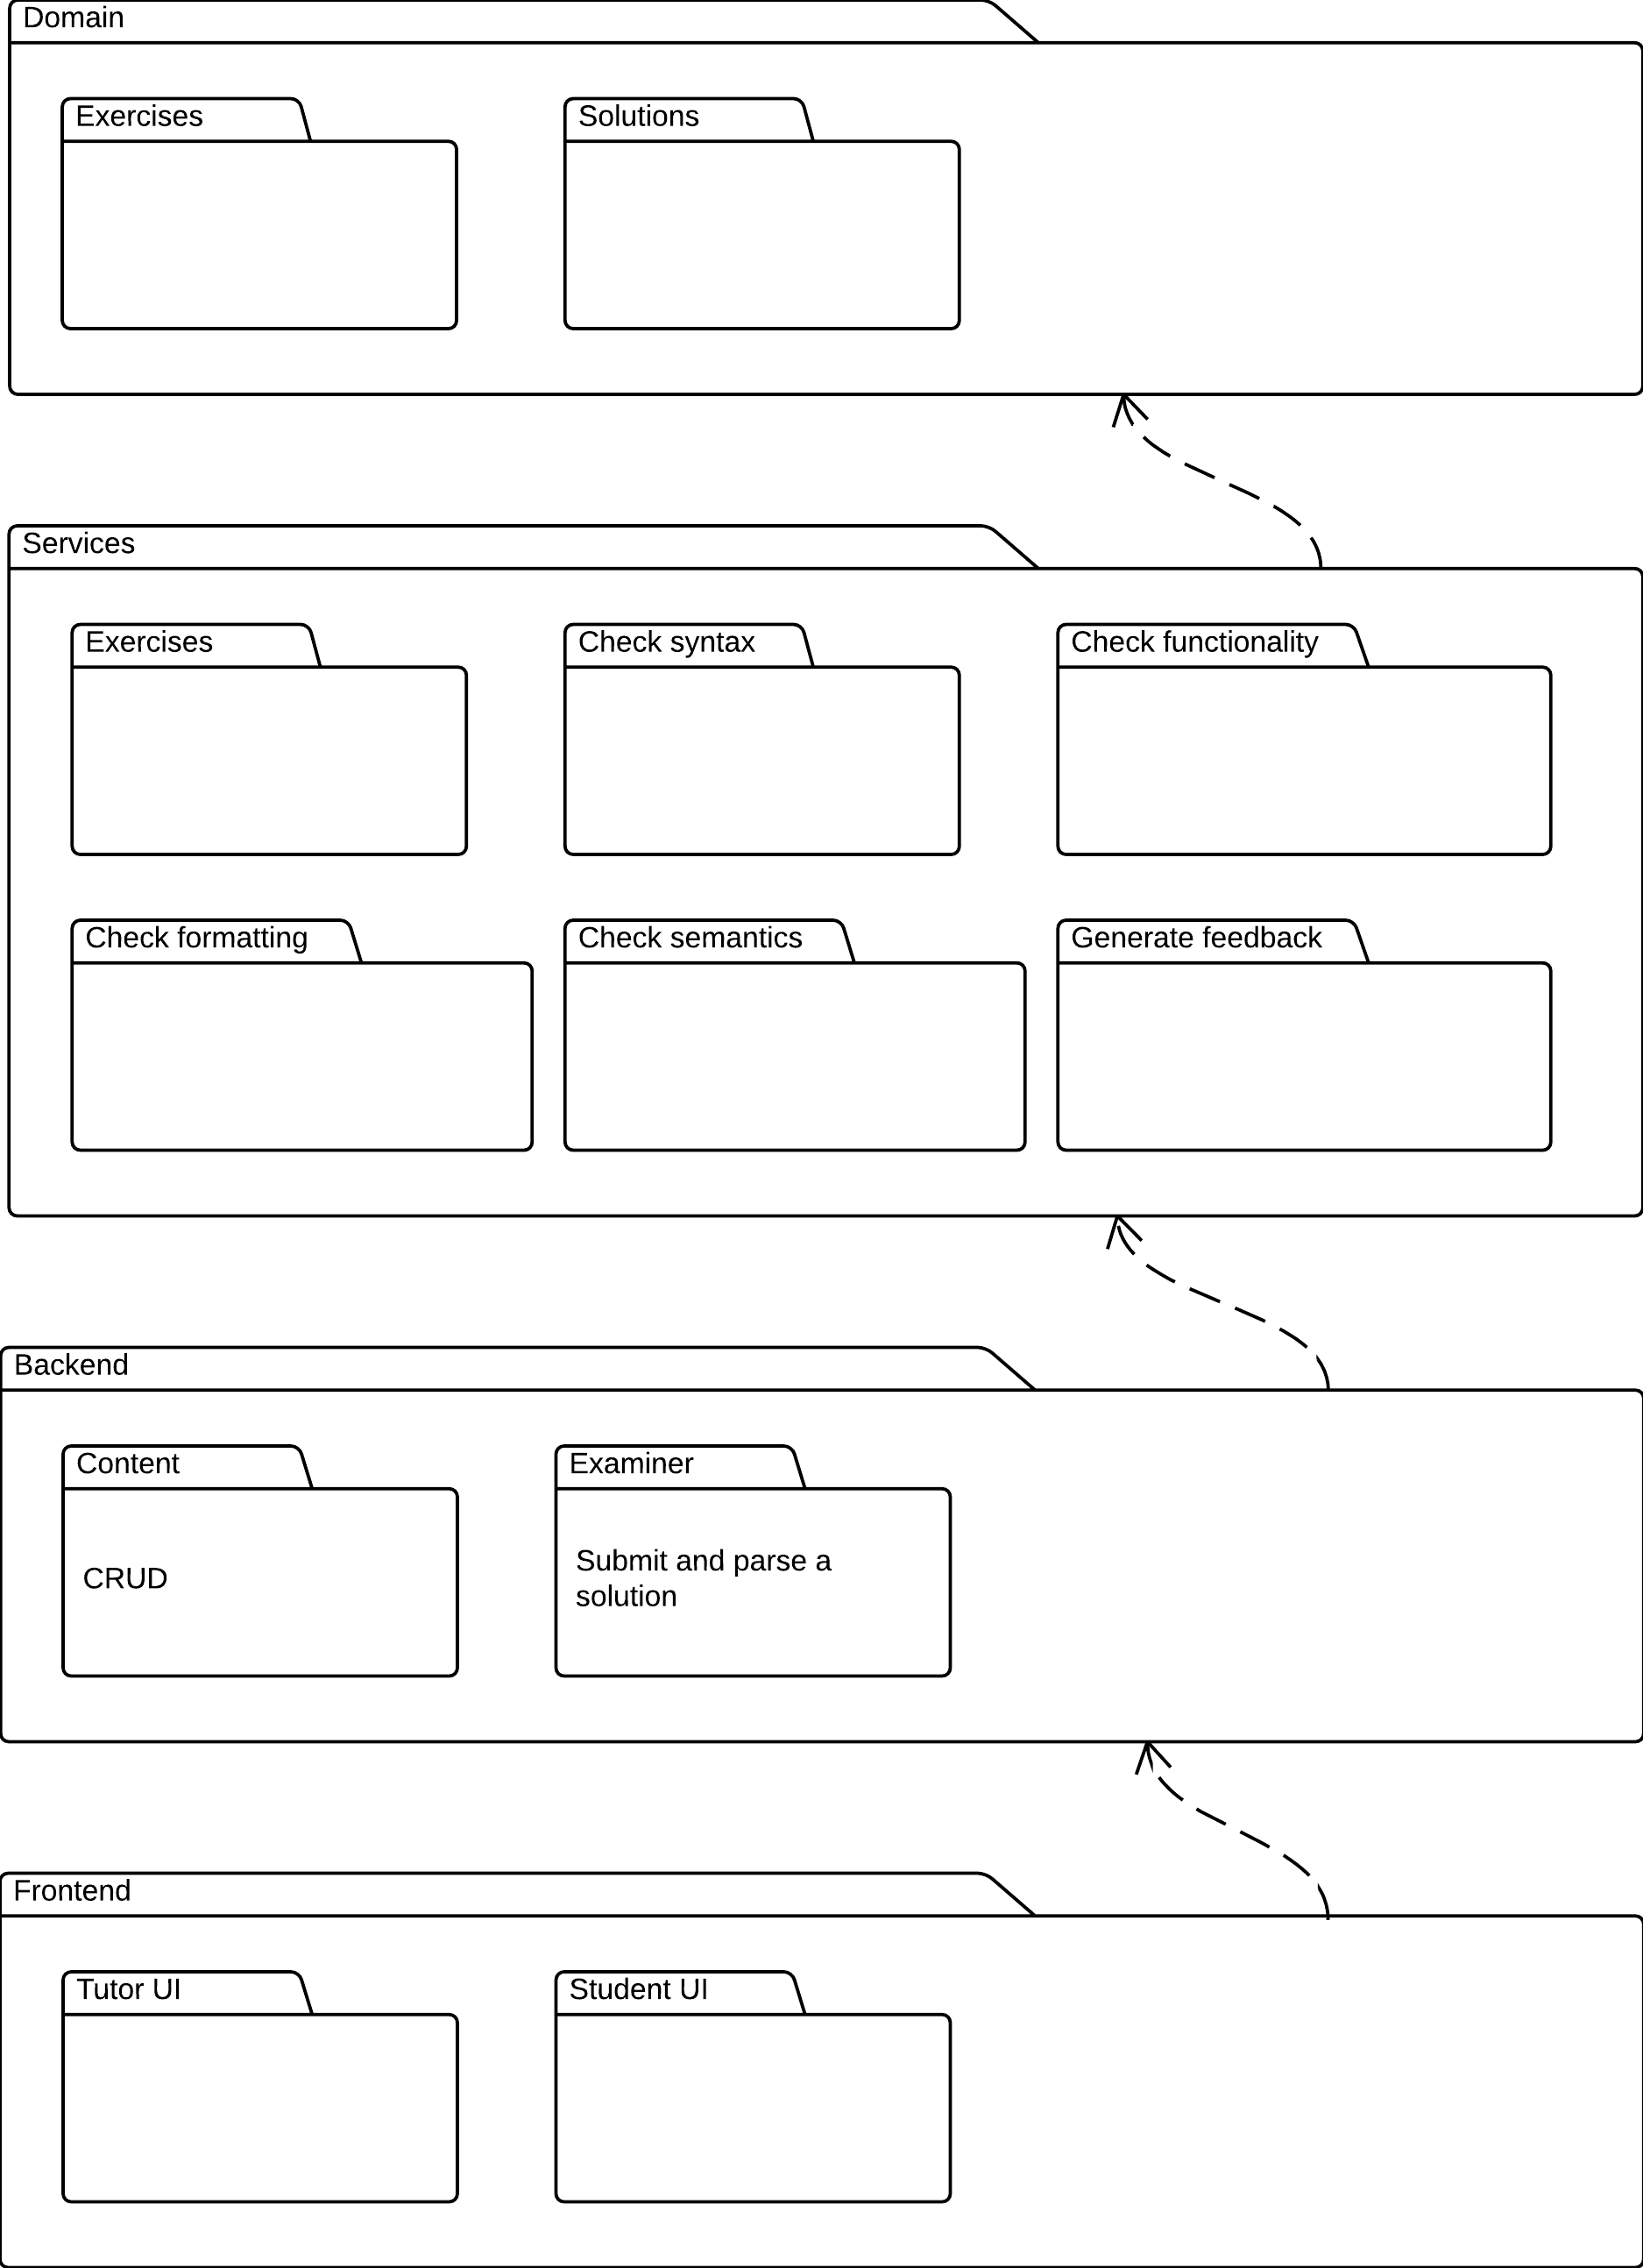
\includegraphics[scale=0.55] {diagrams-images/architecture}

For any future development of this project
the domain can be expanded
and services can be added
without the need to make complex changed to the existing code base.
Only the backend \gls{source-code} needs change
to make use of the added domain data and services.

To structure or own \gls{source-code}
we looked into using a so called ``seed project''.
This is a default template code base and file and folder structure
to get started quickly and relieving you from developing your own architecture.
We found the project
Ultimate-Seed\footnote{\url{https://github.com/pilwon/ultimate-seed}}
which looked promising.
But after a closer examination we concluded it was outdated
and would require to much effort to get to know the full workings,
update and use for the \gls{project}.
So we decided to start from scratch,
concerning the architecture of our own code base.
This way we know exactly what we have,
and we only add code and dependencies when we really need them.
Our code base will be kept clean, small and organized.
And everything will be documented for future teams to get started easily.


\section{Domain Model}
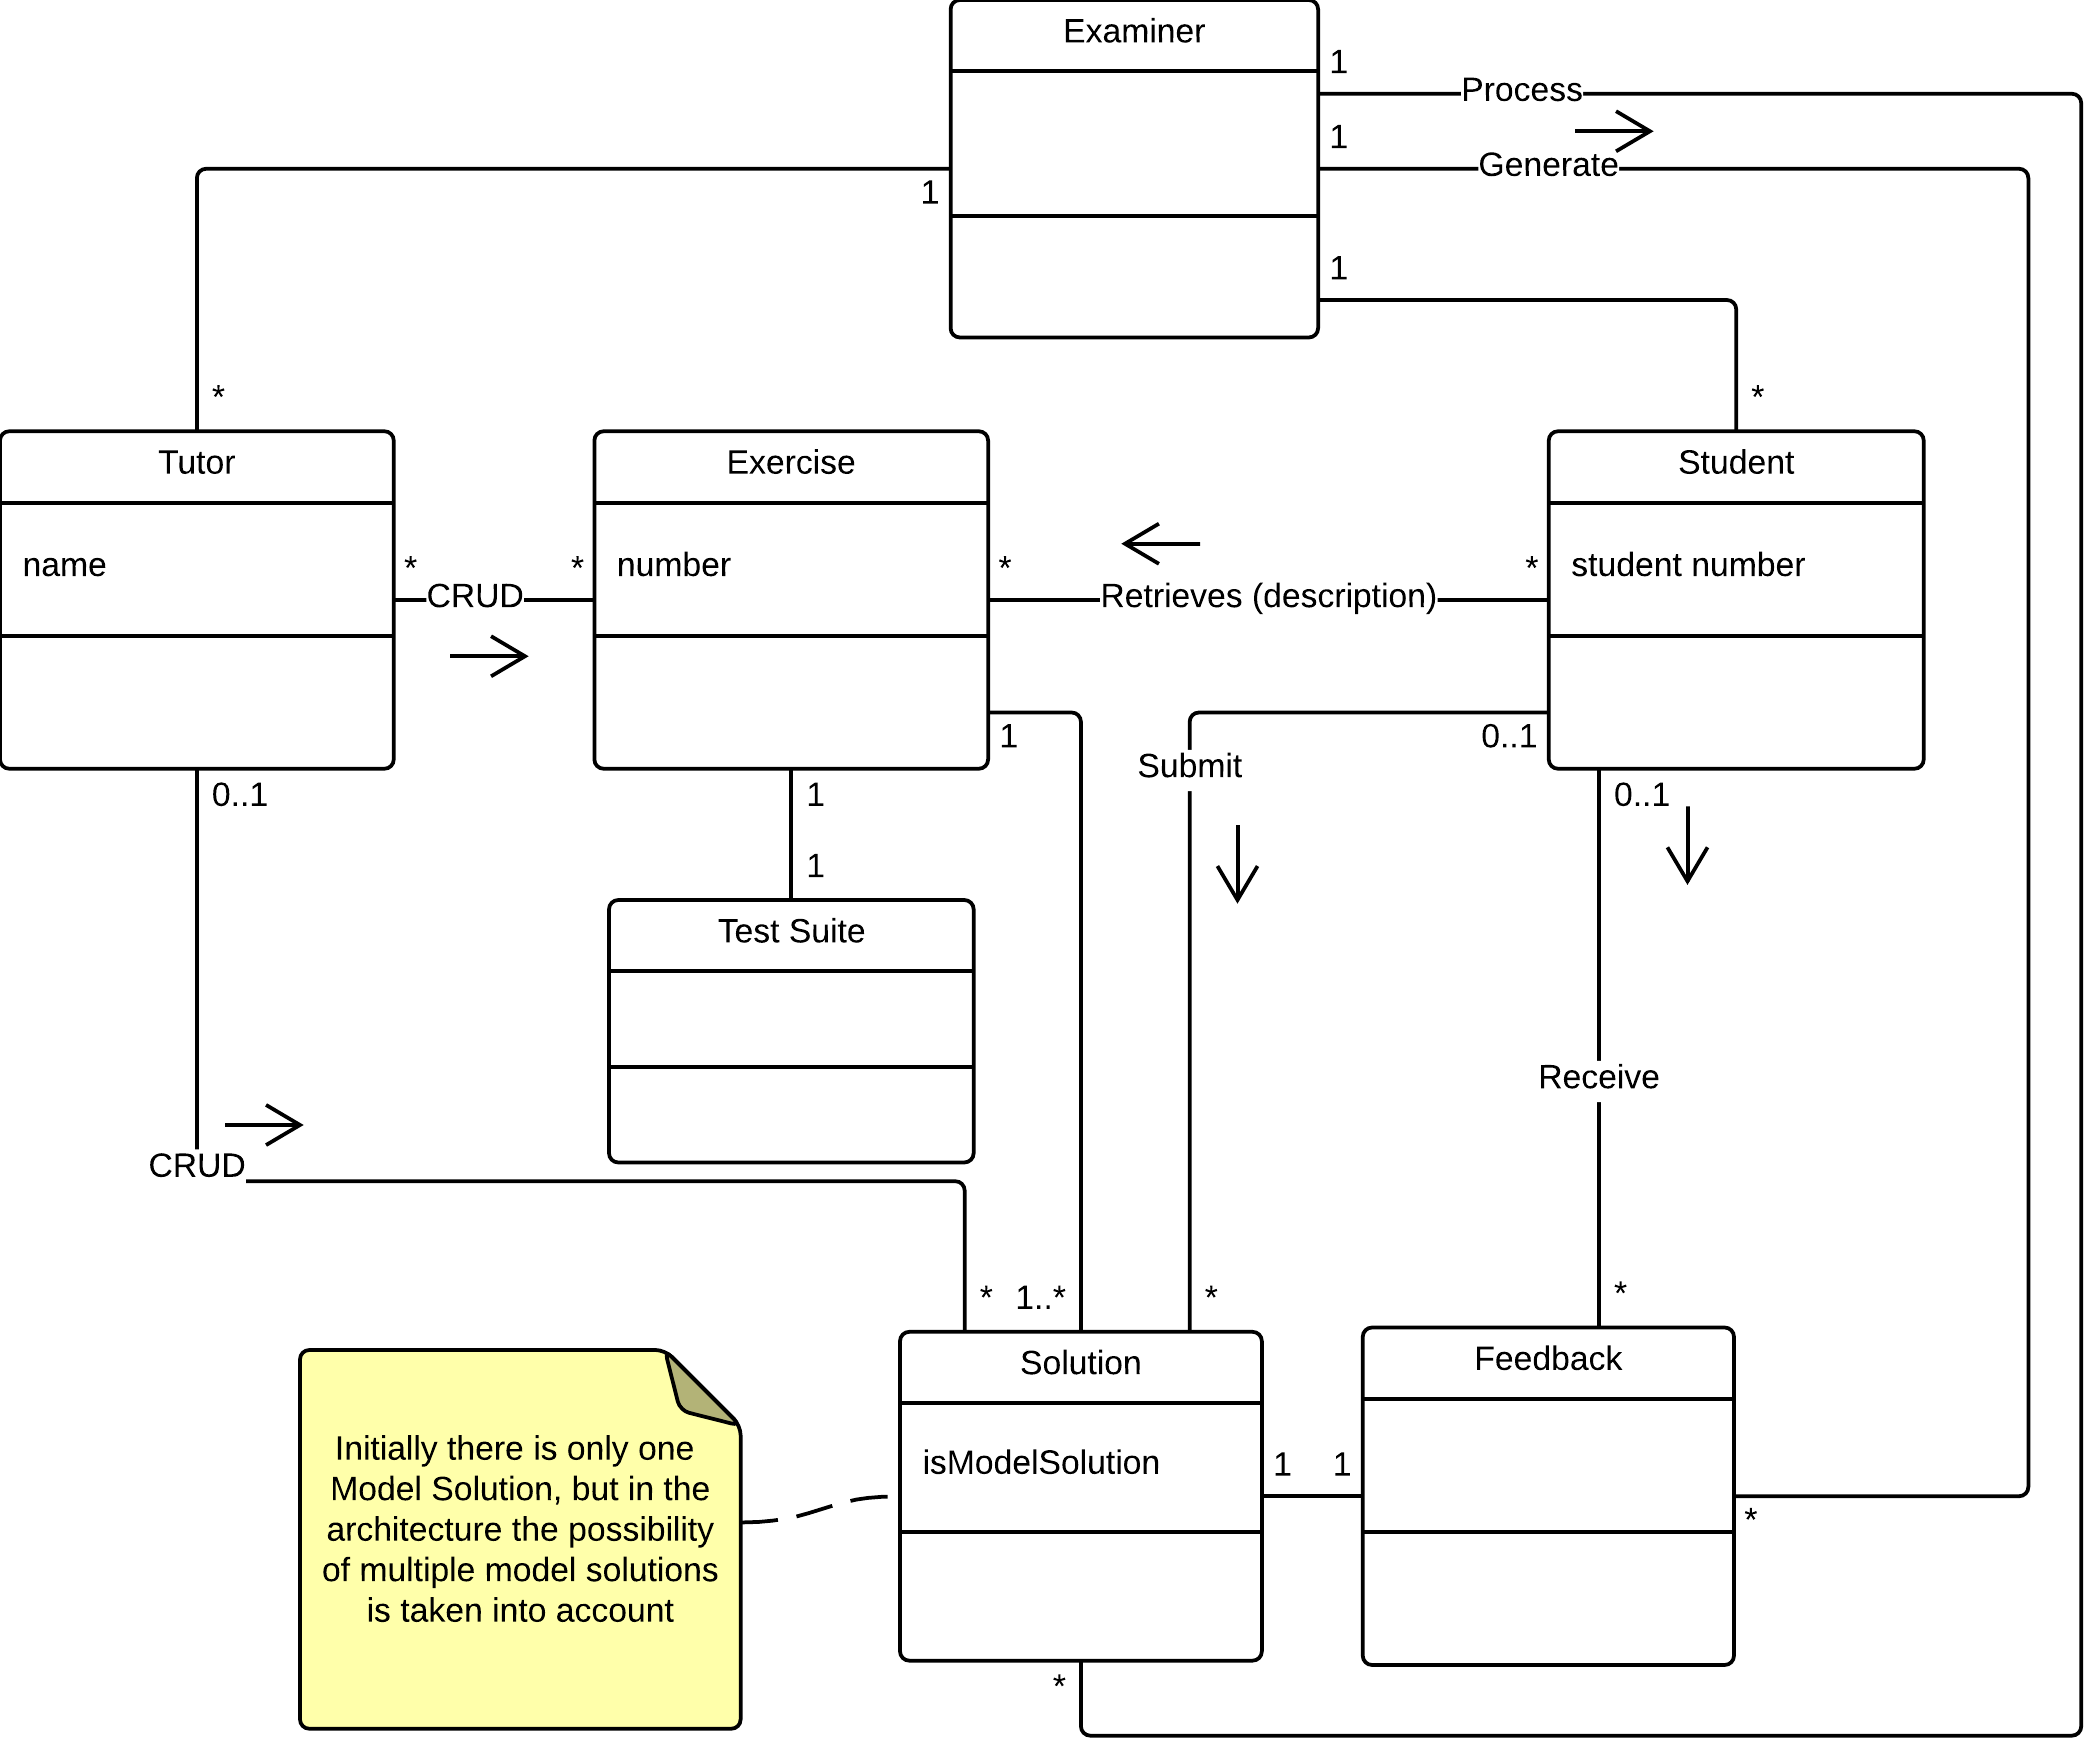
\includegraphics[scale=0.8]{diagrams-images/domain-model}

\section{Use Cases}

\subsection{Use Case Diagram}
% 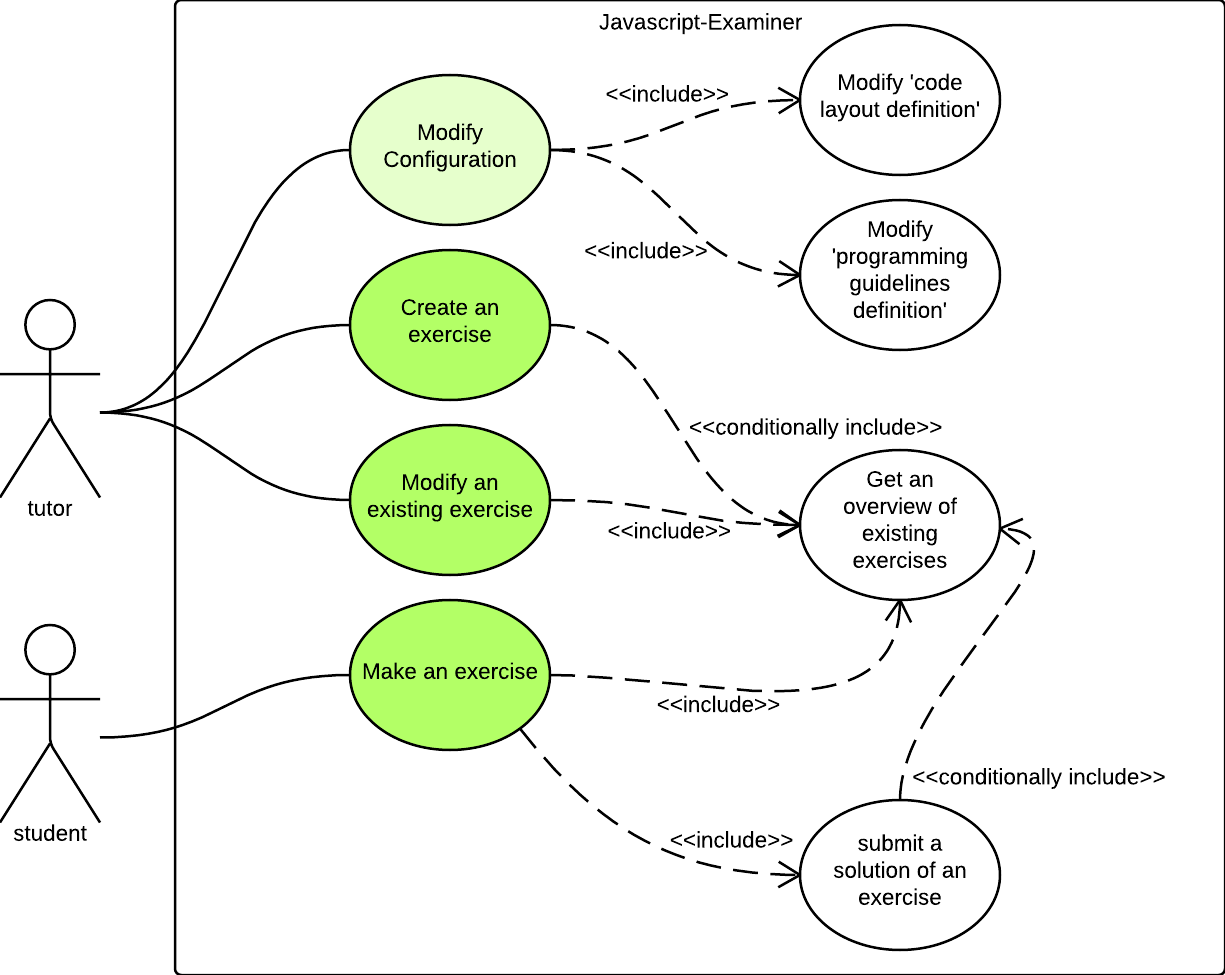
\includegraphics[scale=1.2]{diagrams-images/use-case-diagram}

\subsection{Main Use Cases}

\subsubsection{Create an Exercise}
\begin{mdframed} [rightmargin=-100pt]
\begin{description}
  \item[Scope] Javascript-Examiner
  \item[Level] user goal
  \item[Primary Actor] Tutor
  \item[Preconditions] -
  \item[Success Guarantee] The tutor has created an exercise.
  \item[Main Success Scenario] \mbox{}
	\begin{enumerate}
	  \item Tutor starts creation of a new exercise.
	  \item System requests general exercise information.
	  \item Tutor provides general exercise information.
    \item System request model solution(s).
    \item Tutor provides model solution(s).
    \item System requests test suite.
    \item Tutor provides test suite.
    \item System shows overview with exercise information.
    \item Tutor acknowledges exercise information.
    \item System confirms the exercise is successfully added.
	\end{enumerate}
\end{description}
\end{mdframed}

\subsubsection{Modify an Exercise}
\begin{mdframed} [rightmargin=-100pt]
\begin{description}
  \item[Scope] Javascript-Examiner
  \item[Level] user goal
  \item[Primary Actor] Tutor
  \item[Preconditions] There is at least 1 exercise available.
  \item[Success Guarantee] The tutor has modified an exercise.
  \item[Main Success Scenario] \mbox{}
	\begin{enumerate}
	  \item Tutor selects exercise from overview. \underline{Include: get
        an overview of available exercises}
	  \item System presents editable overview with exercise information.
	  \item Tutor modifies exercise information.
    \item Tutor submits modified exercise information.
    \item System confirms the exercise is successfully modified.
	\end{enumerate}
\end{description}
\end{mdframed}

\subsubsection{Make an exercise}
\begin{mdframed} [rightmargin=-100pt]
\begin{description}
  \item[Scope] Javascript-Examiner
  \item[Level] user goal
  \item[Primary Actor] Student
  \item[Preconditions] There is at least 1 exercise available.
  \item[Success Guarantee] Student has received feedback on the submitted 
	solution.
  \item[Main Success Scenario] \mbox{}
	\begin{enumerate}
	  \item Student selects exercise from overview. \underline{Include: get
        an overview of available exercises}
	  \item Student requests exercise instruction.
	  \item System presents exercise instruction.
	  \item Student submits solution. \underline{Include: submit a solution of 
	    an exercise}
	  \item System presents feedback
	\end{enumerate}
\end{description}
\end{mdframed}

\subsubsection{Modify configuration}
\newpage
\subsection{Supporting Use Cases}

\subsubsection{Get an overview of existing exercises}
\begin{mdframed} [rightmargin=-100pt]
\begin{description}
  \item[Scope] Javascript-Examiner
  \item[Level] Subfunction
  \item[Primary Actor] Student, Tutor
  \item[Preconditions] Usecase \underline{make an exercise}, 
							   \underline{create an exercise} or
							   \underline{modify an exercise} initiated.
  \item[Success Guarantee] An overview of available exercises is 
    presented.
  \item[Main Success Scenario] \mbox{}
    \begin{enumerate} 
	  \item Student / Tutor requests overview of exercises
	  \item System presents overview of exercises
	\end{enumerate}
  \item[Extensions] \mbox{}
    \begin{enumerate}
	  \renewcommand{\labelenumi}{\theenumi a.}
	  \item Only a selection of the exercises is being requested:
		\begin{enumerate}[(1)]
		  \renewcommand{\labelenumii}{\theenumii .}
		  \item Student/Tutor provides a search string.
		  \item System presents the selection of exercises.
		\end{enumerate}
	\end{enumerate}
\end{description}
\end{mdframed}

\subsubsection{Submit the solution of an exercise}
\begin{mdframed} [rightmargin=-100pt]
\begin{description}
  \item[Scope] Javascript-Examiner
  \item[Level] Subfunction
  \item[Primary Actor] Student
  \item[Preconditions] Usecase \underline{make an exercise} initiated.
  \item[Success Guarantee] The solution has been submitted, the student has been
    provided with feedback.
  \item[Main Success Scenario] \mbox{}
    \begin{enumerate}
		\item Student requests submission of the solution.
		\item System requests the solution.
		\item Student submits the solution.
		\item System presents feedback on solution.
    \end{enumerate} 
  \item[Extensions] \mbox{}
	\begin{enumerate}
      \renewcommand{\labelenumi}{\theenumi a.}
	  \item The interaction with the system has been interupted:
		\begin{enumerate}[(1)]
		  \renewcommand{\labelenumii}{\theenumii .}
		  \item Student selects corresponding exercise from overview. \\
		    \underline{Include: get an overview of available exercises}
		  \item System shows options for selected exercise.
		  \item Student requests submission of the solution.
		\end{enumerate}
	\end{enumerate}
\end{description}
\end{mdframed}

\section{Activity Diagrams}
\subsection{Code Submission}
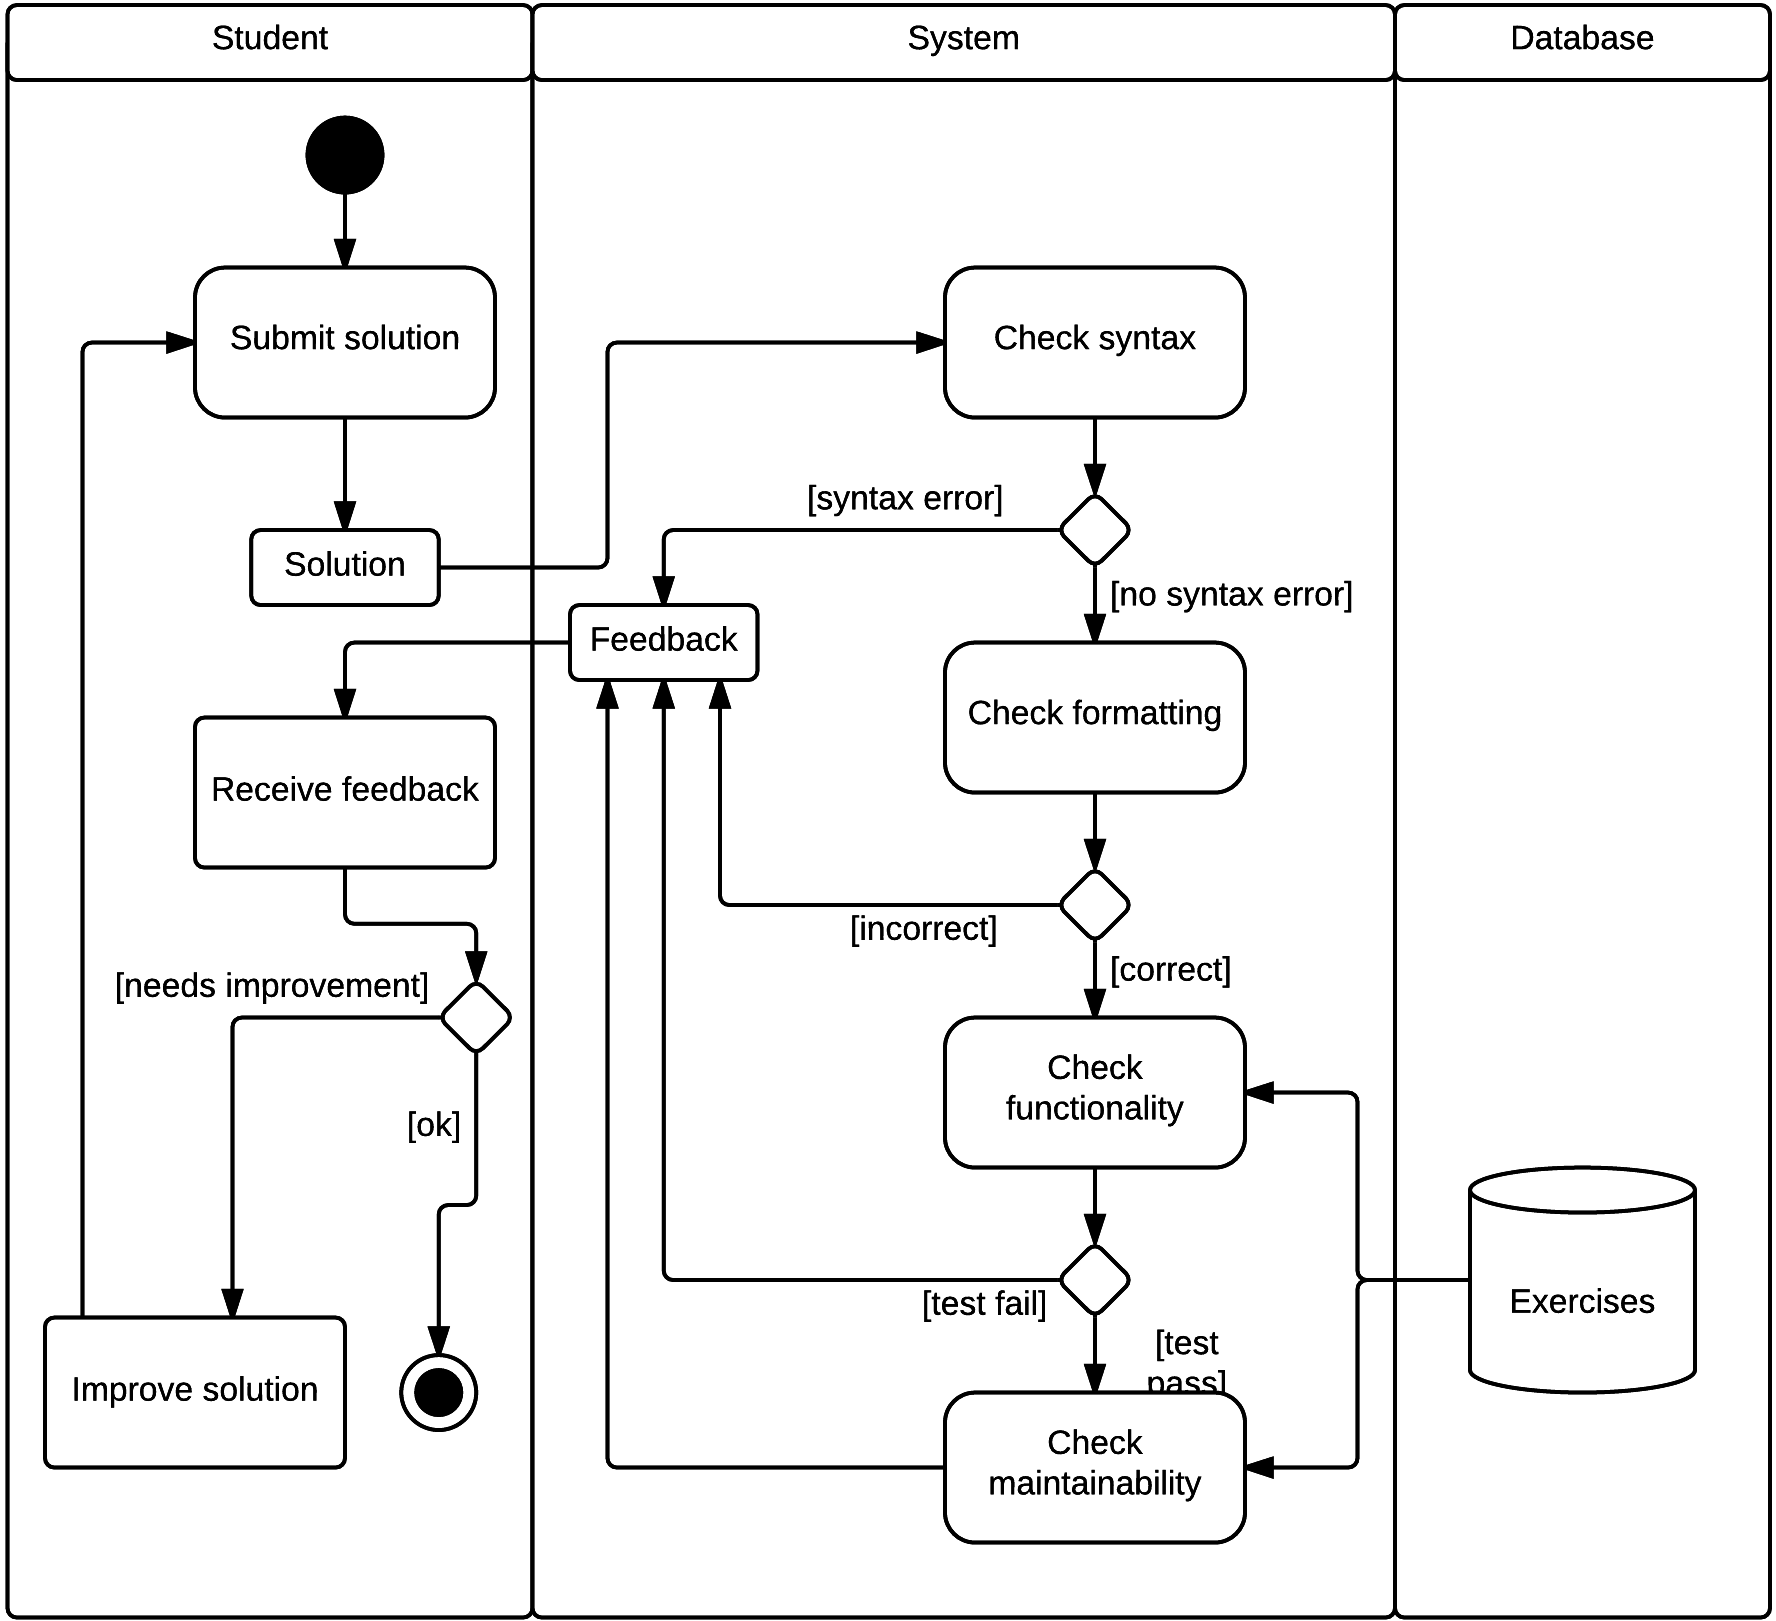
\includegraphics[scale=0.8]{diagrams-images/code-submission-activity-diagram}

